\subsection{Model}

We consider a network of known nodes ($\mathcal{N}$) with access to a shared, public broadcast channel ($\mathcal{B}$), which nodes may \texttt{broadcast()} into and \texttt{listen()} to. The communications primitives our model relies upon are shown in Alg.~\ref{alg:comms_primitive}.

Network nodes \textsc{Bid} to participate in consensus by announcing transaction \texttt{id}s with their required consensus set size. The network forms consensus on the set of nodes and bids to accept, thereby establishing the global key $\mathcal{X}_\mathcal{N}$ which defines the assignment of consensus sets via distributed implementation of the random subset problem.

%\begin{figure}[!htb]
%	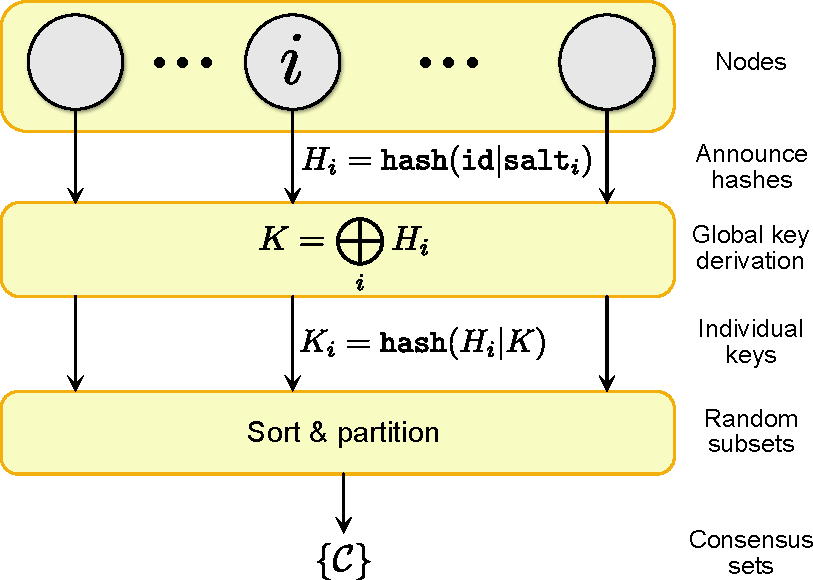
\includegraphics[width=\columnwidth]{figures/hash_based_random_subsets.pdf}
%	\caption{\textbf{Secure distributed random subset algorithm.} Nodes bid by announcing hashes $H_i$. Consensus on valid bids establishes a global key $K$, which is rehashed with all $H_i$ to obtain the local keys $K_i$ used for random assignment.}
%\end{figure}

%\section{Notation}

%$\mathcal{S}_N$, $\mathcal{S}_P$, $\mathcal{S}_C$ denote sets of network ($N$), participating ($P$) and consensus set ($C$) nodes.

%$\mathcal{B}$ denotes a common broadcast channel, observed by all nodes, into which all nodes may announce messages.

%A distributed consensus network comprises a set of known nodes accessing a shared broadcast channel, $\mathcal{B}$. There are two types of nodes, consensus ($\mathcal{C}$) and validator ($\mathcal{V}$) nodes, both bidding to participate in consensus on a bundle of transactions, for which they are offered a reward upon completion.
%
%All nodes possess the same list of public signatures of every node in the network, defining the consensus and validator pools. Nodes are allocated to consensus sets via distributed implementation of the random subset problem. Consensus nodes $\mathcal{C}$ are allocated to forming consensus on statements presented by the market, while validator nodes $\mathcal{V}$ are responsible for enforcing compliance of consensus nodes.
%
%To incentivise compliance with the protocol, nodes initially stake a deposit to participate, returned upon completing the protocol.

%\subsection{Communications primitives}

\begin{algorithm}[H]
	\begin{algorithmic}
		\Function{Announce}{$\mathtt{node}$, $\mathtt{statement}$}
		\State $\mathtt{message} = \textsc{Sign}(\mathtt{node}, \mathtt{statement})$
		\State $\mathcal{B} \gets \mathcal{B} \cup \mathtt{message}$ \Comment{Broadcast}
		\EndFunction
		\State
		\Function{CommitReveal}{$\mathtt{node}$, $\mathtt{statement}$}
		\State $\mathtt{salt} = \textsc{Random}(\{0,1\}^n)$
		\State \LComment{1. Commit hash}
		\State \textsc{Announce}($\mathtt{node}$, $\textsc{Hash}(\mathtt{statement}|\mathtt{salt})$)
		\State \LComment{2. Reveal pre-image}
		\State \textsc{Announce}($\mathtt{node}$, $\mathtt{message}|\mathtt{salt}$)
		\EndFunction
		%\State
		%\Function{Reveal}{$\mathtt{node}$, $\mathtt{statement}$}
		%	\State \textsc{Announce}($\mathtt{node}$, $\mathtt{salt(statement)}$)
		%\EndFunction
	\end{algorithmic}
	\caption{Communications primitives, where $\mathcal{B}$ denotes the shared broadcast channel and numbers denote distinct synchronous steps.} \label{alg:comms_primitive}
\end{algorithm}

\subsection{Protocol}

\begin{figure}[!htb]
	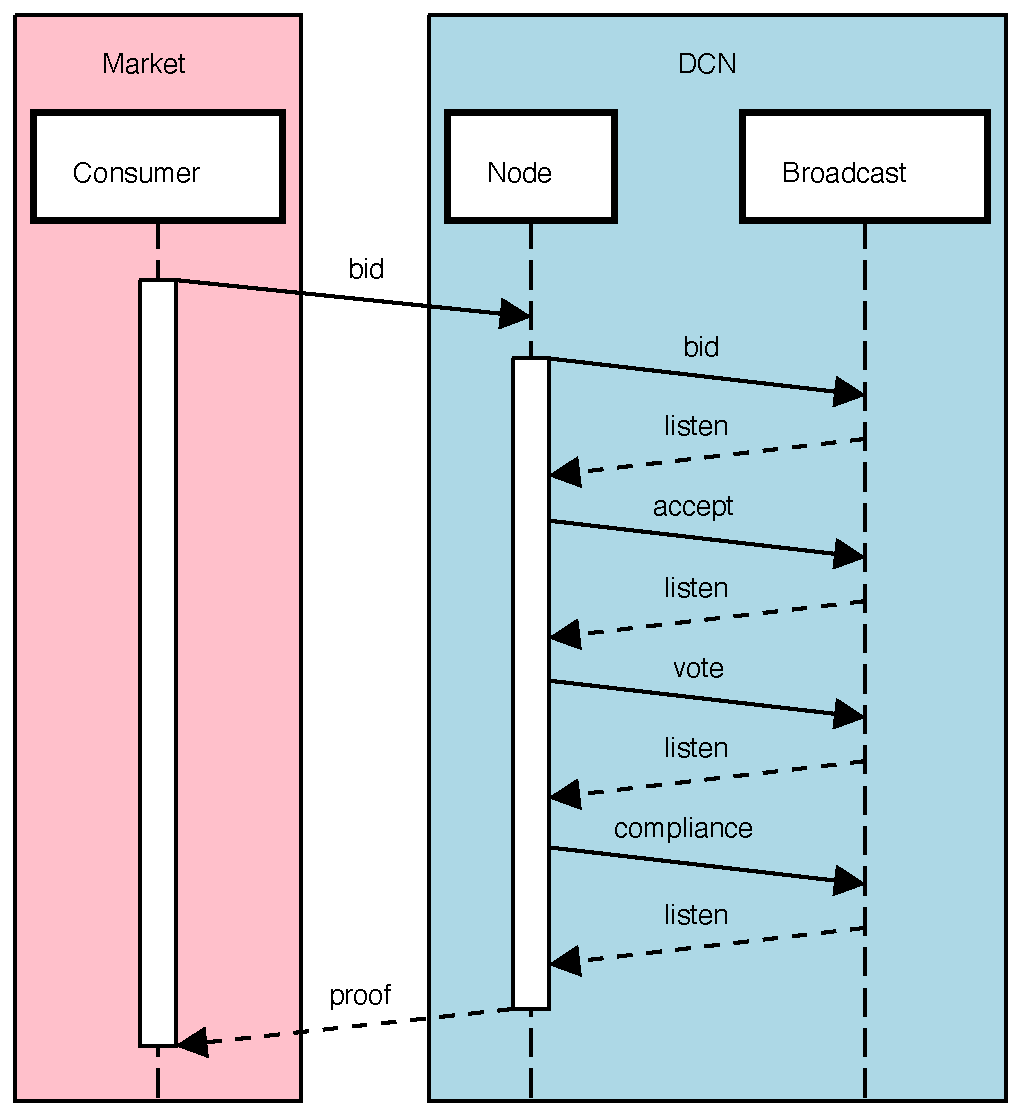
\includegraphics[width=\columnwidth]{figures/sequence_diagram.pdf}
	\caption{\textbf{DCN protocol sequence diagram.} (blue) DCN internal network. (red) External consensus market.} \label{fig:sequence_diagram}
\end{figure}

The DCN protocol is synchronous with the following steps for each network node $i\in\mathcal{N}$:
\begin{enumerate}
	\item \textsc{Bid}: Nodes ($i$) bid to participate by presenting a set of requests ($j$) for consensus sets of given sizes ($|\mathcal{C}_{i,j}|$),
	      \begin{align}
		      \mathcal{R}_{i,j} & = (\mathtt{id}_{i,j},|\mathcal{C}_{i,j}|),\nonumber \\
		      \mathcal{R}_i     & = \bigcup_j \mathcal{R}_{i,j},
	      \end{align}
	      and stating recognised network nodes via the set of their public keys ($\mathtt{PubKey}_j$),
	      \begin{align}
		      \mathcal{N}^{(i)} = \{\mathtt{PubKey}_j\}.
	      \end{align}
	      All nodes broadcast (commit-reveal):
	      \begin{align}
		      \mathcal{B} \gets (\mathcal{R}_i, \mathcal{N}^{(i)}).
	      \end{align}
	\item \textsc{Accept}: Observing the broadcast channel $\mathcal{B}$, all nodes infer the accepted network state, bids and participating nodes ($\mathcal{N}'$),
	      \begin{align}
		      \mathcal{B}                                & \to (\tilde{\mathcal{R}},\tilde{\mathcal{N}}',\tilde{\mathcal{N}}),\nonumber \\
		      \tilde{\mathcal{N}}                        & = \textsc{MajorityVote}(\{\mathcal{N}^{(j)}\}),\nonumber                     \\
		      (\tilde{\mathcal{R}},\tilde{\mathcal{N}}') & = \textsc{Accept}(\{\mathcal{R}_j\}),
	      \end{align}
	      where \textsc{Accept}($\cdot$) is a network-agreed deterministic function, and ${}^\sim$ denotes values inferred from the broadcast channel.

	      In this step consensus is performed at the network level where all network nodes form a single consensus set, requiring that participants form a network majority,
	      \begin{align}
		      |\mathcal{N}'|>\frac{|\mathcal{N}|}{2}.
	      \end{align}
	      All other votes in the protocol are conducted at the level of assigned consensus sets.
	      %	 Nodes vote on accepted bids in accordance with network policy, defining the set of participating nodes $\mathcal{S}_P$ and bids $\mathcal{R}$. Agreement on accepted bids implies the established global key $X_{\mathcal{S}_P}$ and assignment of random subsets.
	      %\item $\mathcal{N}_i\in\{\mathtt{public\_key}\}^{|\mathcal{S}|}$, $\mathcal{P}_i\in\{0,1\}^{|\mathcal{S}|}$: List of public-keys of all recognised network nodes, and associated binary vector of recognised participants.
	\item \textsc{Consensus}: The global key $\mathcal{X}_{\mathcal{N}}$ is implied by the accepted parameters (Sec.~\ref{sec:secure_shared_randomness}) as is the network's allocation to consensus sets via the random subset algorithm (Sec.~\ref{alg:random_subset}).
	      \begin{align}
		      \mathcal{B} & \to \mathcal{X}_{\mathcal{N}} \to \{\mathcal{C}\}.
	      \end{align}
	      Participating nodes vote (commit-reveal) on their assigned consensus requests,
	      \begin{align}
		      \mathcal{B} & \gets \textsc{Vote}_i(\tilde{\mathcal{R}}).
	      \end{align}
	\item \textsc{Compliance}: Nodes vote (announce) on the compliance of participating nodes and reveal the time-of-receipt of all broadcast messages associated with the respective consensus'. Compliant nodes follow all required protocol steps, are in agreement with the majority on all votes, where timestamps (time-of-receipt) of all announcements are within the network's $\delta$ threshold.
	      \begin{align}
		      \mathcal{B} \gets \textsc{CompliantSet}_i(\mathcal{N}).
	      \end{align}
\end{enumerate}
% , \textsc{Timestamp}_i(\mathcal{B})

%A synchronous protocol for solving the random subset problem is shown in Alg.~\ref{alg:consensus_sets}, where numbers indicate the synchronous steps.

%Nodes must remain compliant with the protocol to secure return of their stake. This requires nodes to be in agreement with the majority on all votes. For validator nodes this additionally requires their timestamps of messages in the broadcast channel be consistent with consensus time, where all validator nodes are required to timestamp all messages in the broadcast channel.

%The consensus time for a given message is taken to be the median of all reported timestamps. The median exhibits the property that if a majority of timestamps are within $\delta$ of the median, no action by an adversarial minority is able to undermine this. Hence, consensus time is dictated by the majority. In a setting where non-compliance is penalised, this incentivises consensus time towards accuracy, allowing the protocol to self-synchronise, independent of an external time reference.

%\begin{algorithm}[!htb]
%\begin{algorithmic}
%\Function{ConsensusSets}{$\mathcal{S}$, $\{|C|\}$, $\{\texttt{id}\}$} $\to \{\mathcal{C}\}$
%	\State \LComment{1. Nodes bid to participate}
%	\For{$i\in \mathcal{P}$}
%		\LComment{Announce salted hash of \texttt{header}}
%		\State $H_i \gets \textsc{Commit}(i, \mathtt{header})$
%	\EndFor
%%	\State
%%	\State \LComment{2. Validators commit recognised bids}
%%	\For{$j\in \mathcal{S}_V$} 
%%		\State $B_j \gets \textsc{Commit}(j, \textsc{RecognisedBids}(j))$
%%	\EndFor
%	\State
%	\State \LComment{2. Nodes form consensus on valid bidders}
%	\State $A \gets \textsc{ConsensusParticipants}(\mathcal{P})$
%	\State
%	\State \LComment{3. Assign consensus sets}
%	\State $K = \textsc{Hash}(\textsc{Sort}(\bigcup_{i\in A} H_i))$ \Comment{Shared randomness}
%	\For{$i\in A$}
%	\State $K_i \gets \textsc{Hash}(H_i|K)$ \Comment{Randomised local keys}
%	\EndFor
%	\State $\mathtt{sorted} \gets \textsc{Sort}(A, \{K_i\})$ \Comment{Sort nodes by local keys}
%	\State $\mathcal{C} \gets \textsc{Partition}(\mathtt{sorted}, N_C)$ \Comment{Partition into sets}
%	\State \Return $\mathcal{C}$
%\EndFunction
%\end{algorithmic}
%\caption{Distributed synchronous protocol for hash-based random subsets.} \label{alg:consensus_sets}
%\end{algorithm}

%\begin{algorithm}[!htb]
%\begin{algorithmic}
%\Function{Compliance}{$\mathcal{S}$} $\to \tilde{\mathcal{S}}$
%	\State $\tilde{\mathcal{S}} \gets \{\}$ \Comment{Compliant nodes}
%	\For{$j\in \mathcal{S}$}
%		\State $\mathtt{compliant} \gets \mathtt{true}$
%		\State
%		\State \LComment{Nodes must agree with majority votes}
%		\State $\mathcal{C} \gets \textsc{ConsensusParticipants}(\mathcal{V})$
%		\State $\mathcal{C}_j \gets \textsc{RecognisedParticipants}(j)$
%		\If{$\mathcal{C} \neq \mathcal{C}_j$}
%			\State $\mathtt{compliant} \gets \mathtt{false}$
%		\EndIf
%		\State
%		\State \LComment{Nodes must conform with consensus time}
%		\For{$\mathtt{message} \in \textsc{AllMessages}$}
%		\State $t$ = \textsc{Timestamp}($j$, $\mathtt{message}$)
%		\If{$|t -\textsc{ConsensusTime}(\mathcal{V},\mathtt{message})|\geq\delta$}
%			\State $\mathtt{compliant} \gets \mathtt{false}$
%		\EndIf
%		\EndFor
%		\State
%		\If{$\mathtt{compliant}$}
%			\State $\tilde{\mathcal{V}} \gets \tilde{\mathcal{V}} \cup j$
%		\EndIf
%	\EndFor
%	\State \Return $\tilde{\mathcal{V}}$
%\EndFunction
%\end{algorithmic}	
%\caption{Compliance checking.} \label{alg:compliance}
%\end{algorithm}

%\subsubsection{Consensus load allocation}
%
%During bidding nodes ($i$) request some number of independent consensus sets $|\mathcal{R}_i|$, each of size $|\mathcal{C}_{i,j}|$, with net requested consensus load,
%\begin{align}
%	|\mathcal{C}_i| = \sum_{j=1}^{|\mathcal{R}_i|} |\mathcal{C}_{i,j}|.
%\end{align}
%As all consensus sets are subsets of the network, nodes cannot be assigned to a given consensus set more than once, imposing the constraint,
%\begin{align}
%	|\mathcal{C}_{i,j}|\leq |\mathcal{S}_P|.
%\end{align}
%The total consensus load is,
%\begin{align}
%	|\mathcal{C}| = \sum_{i=1}^{|\mathcal{S}_P|} |\mathcal{C}_{i,j}|,
%\end{align}
%which must be allocated within a finite number of network rounds ($N_R$),
%\begin{align}
%	|\mathcal{C}| \leq N_R \cdot |\mathcal{S}_P|.
%\end{align}
%
%In accordance with network-defined policy some subset of bids are \textsc{Accept}ed to bound total consensus load and ensure fairness in access to consensus.

\subsubsection{Voting}

* Assume the network composition is,
\begin{align}
	N=N_H+N_D,
\end{align}
where $N_H>N_D$.

* A network majority requires, 
\begin{align}
	N_\mathrm{maj} = \lfloor N/2\rfloor+1,
\end{align}
votes.

* Requiring at least,
\begin{align}
	N_V = N_\mathrm{maj} + N_D,
\end{align}
votes guarantees the inclusion of $N_\mathrm{maj}$ honest votes, thereby upholding network integrity (correctness?). %Dishonest nodes are not able to inhibit a vote outcome as honest quorum necessarily exists.

* Requiring at least,
\begin{align}
	N_P &= N_V + N_D \nonumber\\
	&= N_\mathrm{maj} + 2 N_D,
\end{align}
participants (i.e bidders) guarantees at least $N_V$ honest voters amongst them, ranging between $N_V$ (all of whom are honest) to $N_P$ ($N_V$ honest + $N_D$ dishonest).

* Since there are at least $N_V$ honest participants, reaching quorum does not rely on dishonest parties who therefore do not have the ability inhibit quorum.

* Treating all dishonest votes as ambiguous ($\bot$) and honest votes as known with $N_H = N_+ + N_-$ votes for ($+$) and against ($-$) \textsc{Accept}.

* Here $0\leq N_+ \leq N_D$ is a subjective value.

* A simple majority vote will be ambiguous when,
\begin{align}
	N_\mathrm{maj} - N_D < N_+ < N_\mathrm{maj}\nonumber\\
\end{align}
Within this window dishonest voters may swing the simple-majority outcome in either direction.
If dishonest votes are in favour we have,
\begin{align}
	N_+ + N_D \geq N_\mathrm{maj},
\end{align}
and the outcome is unambiguous \textsc{Accept}.
If dishonest votes go against we have,
\begin{align}
	N_+ < N_\mathrm{maj},
\end{align}
and the outcome is unambiguous \textsc{Reject}.

* When,
\begin{align}
	N_+ + N_D < N_\mathrm{maj},
\end{align}
it is not possible for withheld dishonest votes to swing the outcome to \textsc{Accept} and the result is unambiguous \textsc{Reject}.

* Using three-valued logic the subjective simple majority vote outcome is,
\begin{widetext}
\begin{align*}
	\textsc{MajorityVote}^{(i)}(\cdot) = \begin{cases}
 			0, &N_+^{(i)} < N_\mathrm{maj} - N_D \\
 			1, &N_+^{(i)} \geq N_\mathrm{maj} + N_D\\
 			\bot, &N_\mathrm{maj} - N_D < N_+^{(i)} < N_\mathrm{maj} + N_D
	\end{cases},
\end{align*}
\end{widetext}
where the subjective outcome is relative to a party's understanding of $N_+^{(i)}$.

* As different nodes may have different subjective interpretations of $N_+$, when the majority vote is ambiguous for some it may be unambiguous for others. As honest nodes are compliant all parties have the same subjective understanding of honest vote outcomes. Dishonest nodes may be non-compliant, resulting in fragmentation from inconsistent subjective understanding of their outcomes.

* If a node subjectively believes there are $N_+ \geq N_\mathrm{maj}$ votes to \textsc{Accept}, hence an \textsc{Accept} majority vote outcome, other nodes may subjectively believe there are a minimum of $N_+ - N_D$ votes to \textsc{Accept}. Hence, a voter ($A$) who subjectively observes $N_+^{(A)} \geq N_\mathrm{maj}$ can only be certain other nodes share that understanding when $N_+^{(A)} - N_D \geq N_\mathrm{maj}$.

* Subsequent to a simple majority vote, let us hold a supermajority vote requiring $N_V$ votes to pass. As there are at least $N_V$ honest voters amongst the $N_P$ participants quorum exists.

* If the simple majority vote is unambiguous the supermajority vote is required to reflect that outcome (confirmation). If the simple majority vote is ambiguous this implies $N_\mathrm{maj} - N_D < N_+ < N_\mathrm{maj}$. A supermajority of $N_V$ requires $N_+ + N'_+ \geq N_V$, where $N'_+\leq N_D$ are any unknown dishonest votes that may yet additionally contribute.

In the ambiguous regime, a supermajority of $N_V$ requires,
\begin{align}
	N_+ + N'_+ &\geq N_V, \nonumber\\
	N_+ + N'_+ &\geq N_\mathrm{maj} + N_D, \nonumber\\
	N_+ + N'_+ - N_D &\geq N_\mathrm{maj},
\end{align}

Since $N_+ < N_\mathrm{maj} + N_D$

See Fig.~\ref{fig:voting_pie_chart}

\begin{figure*}[!htp]
	\centering
	\pgfkeys{%
/piechartthreed/.cd,
scale/.code                =  {\def\piechartthreedscale{#1}},
mix color/.code            =  {\def\piechartthreedmixcolor{#1}},
background color/.code     =  {\def\piechartthreedbackcolor{#1}},
name/.code                 =  {\def\piechartthreedname{#1}}}

 \newcommand\piechartthreed[2][]{% 
   \pgfkeys{/piechartthreed/.cd,
     scale            = 1,
     mix color        = gray,
     background color = white,
     name             = pc} 
  \pgfqkeys{/piechartthreed}{#1}
  \begin{scope}[scale=\piechartthreedscale] 
  \begin{scope}[xscale=5,yscale=5] 
     \path[preaction={fill=black,opacity=.8,
         path fading=circle with fuzzy edge 20 percent,
         transform canvas={xshift=2mm, yshift=-5mm*\piechartthreedscale}}] (0,0) circle (1cm);
   \fill[gray](0,0) circle (0.5cm);  
     \path[preaction={fill=white,opacity=.8,
          path fading=circle with fuzzy edge 20 percent,
          transform canvas={xshift=1mm, yshift=-2.5mm*\piechartthreedscale}}] (0,0) circle (0.5cm);
     \pgfmathsetmacro\totan{5} 
     \global\let\totan\totan 
     \pgfmathsetmacro\bottoman{180} \global\let\bottoman\bottoman 
     \pgfmathsetmacro\toptoman{0}   \global\let\toptoman\toptoman 
     \begin{scope}[draw=black,thin]
     \foreach \an/\col [count=\xi] in {#2}{%
     \def\space{ } 
        \coordinate (\piechartthreedname\space\xi) at (\totan+\an/2:0.75cm); 
        \ifdim 180pt>\totan pt 
         \ifdim 0pt=\toptoman pt
            \shadedraw[left color=\col!20!\piechartthreedmixcolor, right color=\col!5!\piechartthreedmixcolor, draw=black,very thin] (0:.5cm) -- ++(0,-0.5mm) arc (0:\totan+\an:.5cm) -- ++(0,0.5mm)  arc (\totan+\an:0:.5cm);
            \pgfmathsetmacro\toptoman{180} 
            \global\let\toptoman\toptoman         
            \else
            \shadedraw[left color=\col!20!\piechartthreedmixcolor, right color=\col!5!\piechartthreedmixcolor, draw=black,very thin](\totan:.5cm)-- ++(0,-0.5mm) arc(\totan:\totan+\an:.5cm) -- ++(0,0.5mm)  arc(\totan+\an:\totan:.5cm); 
          \fi
        \fi   
        \fill[\col!20!gray,draw=black] (\totan:0.5cm)--(\totan:1cm)  arc(\totan:\totan+\an:1cm) --(\totan+\an:0.5cm) arc(\totan+\an:\totan :0.5cm);     
       \pgfmathsetmacro\finan{\totan+\an}
       \ifdim 180pt<\finan pt 
         \ifdim 180pt=\bottoman pt
            \shadedraw[left color=\col!20!\piechartthreedmixcolor, right color=\col!5!\piechartthreedmixcolor, draw=black,very thin] (180:1cm) -- ++(0,-0.5mm) arc (180:\totan+\an:1cm) -- ++(0,0.5mm)  arc (\totan+\an:180:1cm);
            \pgfmathsetmacro\bottoman{0}
            \global\let\bottoman\bottoman
            \else
            \shadedraw[left color=\col!20!\piechartthreedmixcolor, right color=\col!5!\piechartthreedmixcolor, draw=black,very thin](\totan:1cm)-- ++(0,-0.5mm) arc(\totan:\totan+\an:1cm) -- ++(0,0.5mm)  arc(\totan+\an:\totan:1cm); 
          \fi
        \fi
        \pgfmathsetmacro\totan{\totan+\an}  \global\let\totan\totan 
       } 
    \end{scope}
    \draw[thin,black](0,0) circle (0.5cm);
   \end{scope}  
\end{scope}
}

\resizebox{!}{0.65\columnwidth}{
 \begin{tikzpicture}
   \piechartthreed[scale=0.5,
      background color=white,
      mix color=darkgray]
      {40/green,40/red,95/white,185/green}
   \foreach \i in {1,2,4} { \fill (pc \i) circle (.5mm);}
   \draw[darkgray] (pc 1)  -- ++(3.6,0) coordinate (s1) node[anchor=south east] {Honest} node[anchor=north east] {$N_V=N_\mathrm{maj}+N_D$};
   \draw[darkgray] (pc 2)  -- ++(0.5,0.5) coordinate (s2) -- (s2 -| s1) node[anchor=south east] {Dishonest} node[anchor=north east] {$N_D$}; 
   \draw[darkgray] (pc 4) coordinate (s3) -- (s3 -| s1) node[anchor=south east] {Majority} node[anchor=north east] {$N_\mathrm{maj}$};
   \node[darkgray] at (0,2.9cm) {\emph{Voters}};
 \end{tikzpicture}
 }
 \hspace{10pt}
\resizebox{!}{0.66\columnwidth}{
 \begin{tikzpicture}
   \piechartthreed[scale=0.5,
      background color=white,
      mix color=darkgray]
      {80/pink,95/white,145/cyan,40/yellow}
   \foreach \i in {1,3,4} { \fill (pc \i) circle (.5mm);}
   \draw[darkgray] (pc 1)  -- ++(3.1,0) coordinate (s1) node[anchor=south east] {Reject} node[anchor=north east] {$0$};
   \draw[darkgray] (pc 4) coordinate (s2) -- (s2 -| s1) node[anchor=south east] {Unknown} node[anchor=north east] {$\bot$}; 
   \draw[darkgray] (pc 3) coordinate (s3) -- (s3 -| s1) node[anchor=south east] {Accept} node[anchor=north east] {$1$};
     \node[darkgray] at (0,2.9cm) {\emph{Ambiguous vote}};
 \end{tikzpicture}
 }

	\caption{???} \label{fig:voting_pie_chart}
\end{figure*}

 %In the latter case, dishonest voters are not able to exploit subjective differences amongst honest nodes to cause splitting.

* Since $N_P = N_\mathrm{maj} + 2 N_D$ comprises (at most) $N_D$ dishonest parties,
\begin{align}
	\dot{r} &= \frac{N_D}{N_P} = \frac{N_D}{p\cdot N} = \frac{r}{p}
\end{align}

%r' = ND/(p.N) = r/p

%
%Hence, with $N_P$ minimum participation, participation by an honest majority of the network is guaranteed.%, and $N_\mathrm{maj}$ unanimous votes
%
% an honest network majority outcome is guaranteed.



With $N_V$ received votes, it is guaranteed a network majority of $N_\mathrm{maj}$ have cast honest votes.

\subsubsection{Network acceptance}

??? TO DO


Decomposing a network into honest and dishonest nodes,
\begin{align}
	\mathcal{N}   & = \mathcal{N}_H \cup \mathcal{N}_D,\nonumber \\
	N & = N_H + N_D,
\end{align}
the ratios of malicious ($r$) and participating ($p$) nodes in the network are,
\begin{align}
	r = \frac{N_D}{N},\quad p = \frac{N_P}{N},
\end{align}
where $\mathcal{N}'$ are the participating nodes,

In a worst-case adversarial model we assume all dishonest nodes are present in any participating set. The ratio of malicious nodes in the participating set is,
\begin{align}
	r' = \frac{N_D}{p\cdot N} = \frac{r}{p},
\end{align}
modulating the effective ratio of dishonest nodes by the ratio of participating nodes, where \mbox{$p>1/2$} and \mbox{$r<1/2$}. Maintaining \mbox{$r'<1/2$} to ensure an honest majority imposes a lower bound on the participation ratio,
\begin{align}
	p_\mathrm{min} > \mathrm{max}(2r,1/2).
\end{align}

As the effective proportion of dishonest nodes, \mbox{$r'=r/p$}, is a function of the variable network participation rate, $p$, the required consensus set size to maintain $\varepsilon$-security may be algorithmically specified upon acceptance. Now the dynamic minimum consensus set size scales as,
\begin{align}
	N_\mathrm{min}(r/p,\varepsilon),
\end{align}
shown in Fig.~\ref{fig:P_M_p}.

\begin{figure}
	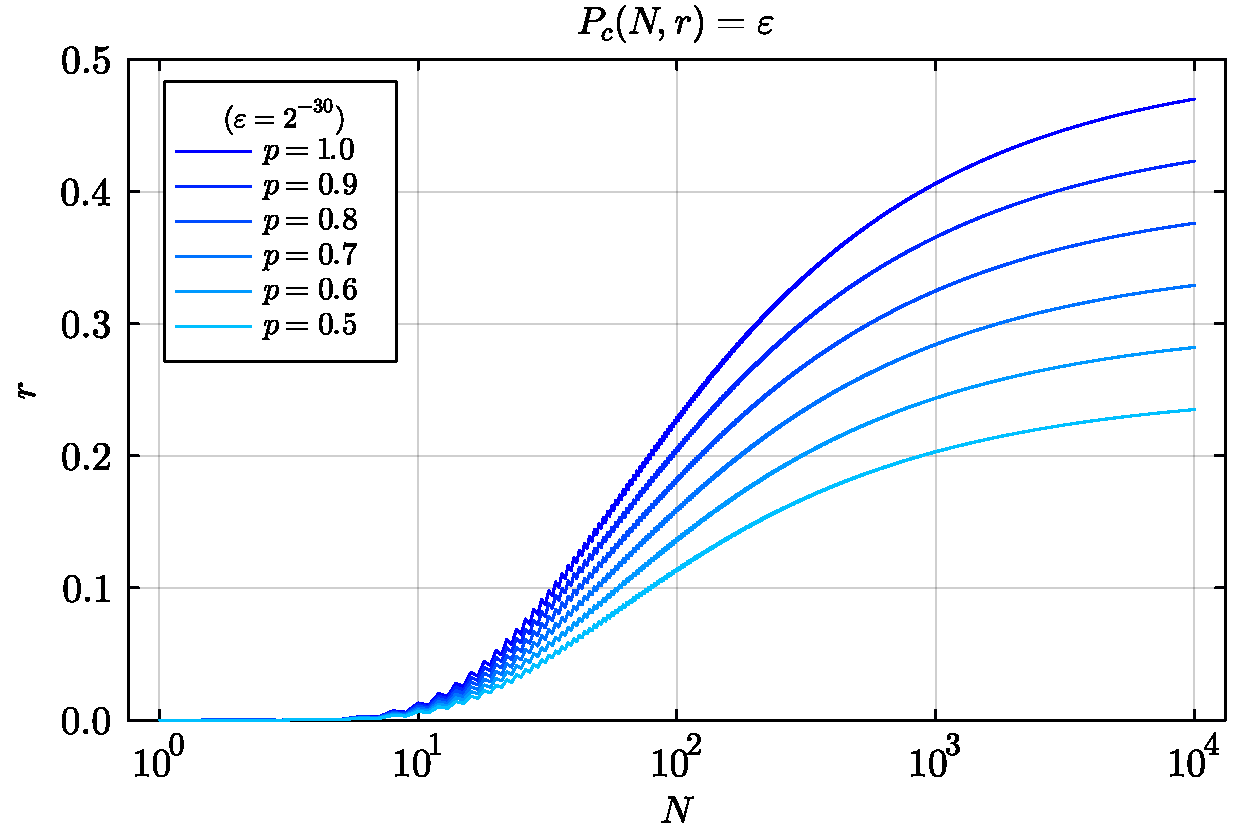
\includegraphics[width=\columnwidth]{figures/majority_prob_p.pdf}\\
	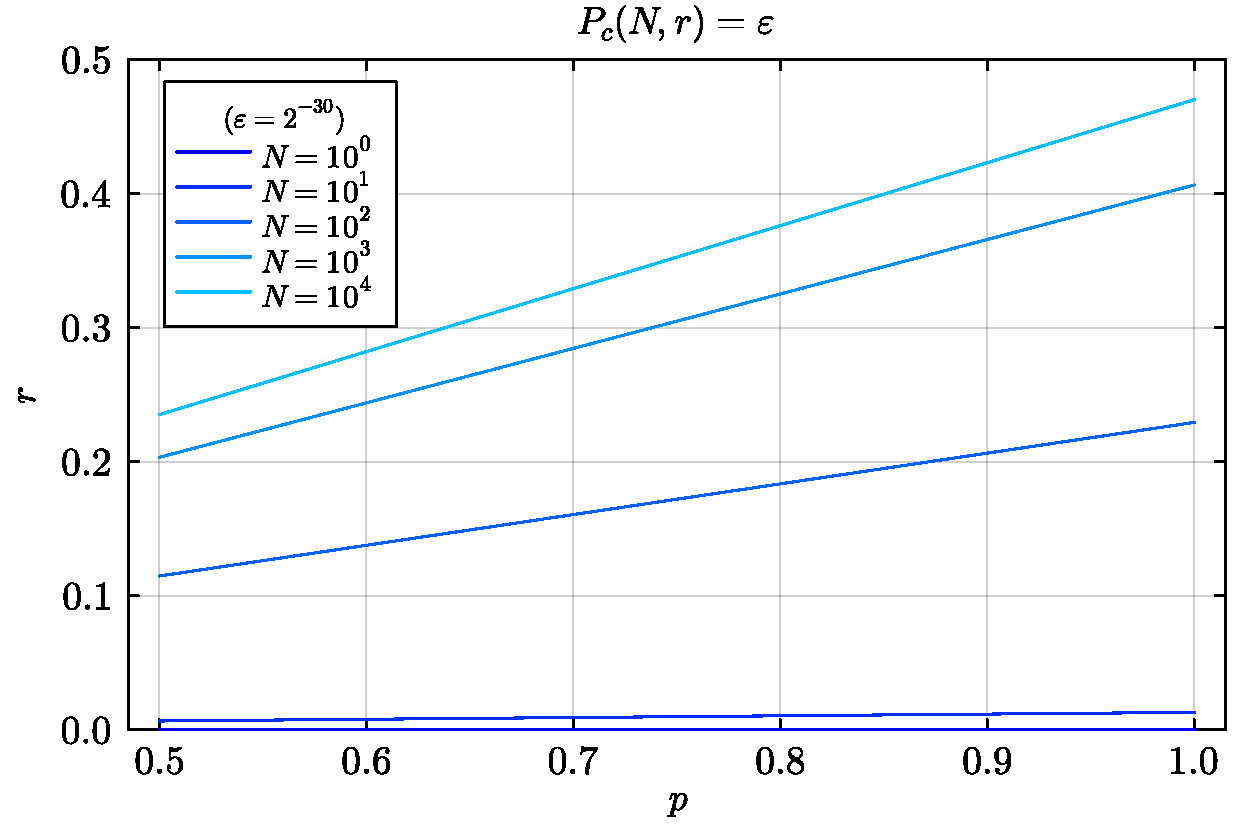
\includegraphics[width=\columnwidth]{figures/majority_prob_N.pdf}
	\caption{\textbf{Security tradeoffs with consensus set size and variable network participation.} \mbox{$P_c(N,r/p)\leq\varepsilon$} is the probability that dishonest nodes within a random subset of size $N$ form a false-majority when the proportion of dishonest nodes is \mbox{$r'=r/p$}, with network participation $p$. Shown for constant \mbox{$\varepsilon=2^{-30}$}, where the \mbox{$p=1$} curve corresponds to the respective curve in Fig.~\ref{fig:P_M}.}\label{fig:P_M_p}
\end{figure}

\subsection{Consensus time}

DEFINITIONS

* Define consensus time of a message broadcast by node $i$ relative to a set of nodes $\mathcal{S}$,
\begin{align}
	\textsc{ConsensusTime}(i,\mathcal{S}) = \mathrm{median}(\{t_{i,j}\}_{j\in\mathcal{S}}),
\end{align}
where $t_{i,j}$ is the reported time-of-receipt of message $i$ by node $j$, and $\{t_{i,j}\}_{j\in\mathcal{S}}$ is the set of reported times-of-receipt of message $i$ by elements of $\mathcal{S}$. 

* Use notation,
\begin{align}
\vec{t}_{i,\mathcal{S}} &= \{t_{i,j}\}_{j\in\mathcal{S}},\nonumber\\
\tilde{t}_{i,\mathcal{S}} &= \mathrm{median}(\vec{t}_{i,\mathcal{S}}).
\end{align}

* For any majority subset,
\begin{align}
	\mathcal{S}_+\subseteq\mathcal{S},\,\,|\mathcal{S}_+|>\frac{|\mathcal{S}|}{2},
\end{align}
we have,
\begin{align}
	\mathrm{min}(\vec{t}_{i,\mathcal{S}_+}) \leq \textsc{ConsensusTime}(i,\mathcal{S}) \leq \mathrm{min}(\vec{t}_{i,\mathcal{S}_+}).
\end{align}
Hence, the consensus-time of a set is bounded by any constituent majority.

* A majority of nodes reporting identical times-of-receipt,
\begin{align}
 	t_{i,j}=t_{i,k} \;\forall\; j,k\in\mathcal{S}_+,
\end{align}
forces convergence of consensus-time,
\begin{align} \label{eq:ct_converge}
	\textsc{ConsensusTime}(i,\mathcal{S}) = t_{i,\mathcal{S}_+},
\end{align}
invariant under times reported by the minority, $\vec{t}_{i,\mathcal{S}_-}$.

PROTOCOL:
\begin{enumerate}
	\item All nodes $i\in\mathcal{S}$ report their times-of-receipt of a given message,
		\begin{align}
			\mathcal{B} \gets t_i,
		\end{align}
	 	and initialise their set of recognised compliant nodes as those whose timestamps subjectively arrived on time,
		\begin{align}
			\mathcal{S}_i^{(0)} = \{j\in\mathcal{S} \,|\, \textsc{ReceivedOnTime}_i(t_{j\to i})\}.
		\end{align}
%	\item Reported $t_{i,j}$ are required to be received within a given window to comply with synchronicity. (talk about tau max constraint).
%	\item Under the latency profile nodes may have different subjective interpretations of which reported times they accept and hence different subjective understandings of consensus-time.
	\item Nodes $i$ record the arrival times of all timestamps announced by $j$ they recognise as compliant ($j\in\mathcal{S}_i$),
		\begin{align}
			\mathcal{B} \to \{t_{j\to i}\}_{j\in \mathcal{S}_i}.
		\end{align}
		and update their set of recognised compliant nodes accordingly,
		\begin{align}
			\mathcal{S}_i^{(n)} = \{j\in\mathcal{S}_i^{(n-1)} \,|\, \textsc{ReceivedOnTime}_i(t_{j\to i})\}.
		\end{align}
		With increasing $n$, subjective subsets of compliant nodes are non-expanding,
		\begin{align}
			\mathcal{S}_j^{(n)} &\subseteq \mathcal{S}_j^{(n-1)}.
		\end{align}
	\item Nodes announce the set of received timestamps they deem compliant (for the $n$th round),
		\begin{align}
			\mathcal{T}_i^{(n)}(S_i^{(n)}) &= \{t_{j\to i}^{(n)}\}_{j\in S_i^{(n)}}, \nonumber\\
				\mathcal{B} &\gets \mathcal{T}_i^{(n)}(S_i^{(n)}).
		\end{align}
		The median of $\mathcal{T}_i^{(n)}(S_i^{(n)})$ is node $i$'s subjective consensus-time.
	\item Nodes $i$ and $j$ mutually recognise the compliance of the set $\mathcal{S}_i \cap \mathcal{S}_j$. Node $i$ interprets the relative consensus-time implied by $j$ via their mutually recognised nodes,
		\begin{align}
			\mathcal{T}_{j\to i}^{(n)} = \mathcal{T}_j^{(n)}(\mathcal{S}_i^{(n)} \cap \mathcal{S}_j^{(n)}).
		\end{align}
%	\item These exhibit pairwise convergence,
%		\begin{align}
%			\mathcal{T}_j^{(n)}(\mathcal{S}_i \cap \mathcal{S}_j).
%		\end{align}
	\item On a pairwise basis relative consensus-times are unambiguous.
	\item Nodes update their sets of timestamps to their new pairwise mutually recognised relative consensus-times,
		\begin{align}
			t_i^{(n)} = \mathrm{median}_j(\mathcal{T}_{j\to i}^{(n)}(\mathcal{S}_i \cap \mathcal{S}_j))
		\end{align}
	\item (Repeat to 1): All nodes announce their updated timestampe,
		\begin{align}
			\mathcal{B} \gets t_i^{(n)}.
		\end{align}
	\item When an majority of nodes $j$ report the same subjective understandings of consensus-time of $i$, all honest nodes necessarily converge (Eq.~\eqref{eq:ct_converge}).
	\item Failure to converge arises when different nodes have different subjective interpretations of consensus-time, which can only occur via minority timing manipulation. This is only possible if when,
		\begin{align}
			\mathcal{S}_j\neq \mathcal{S}_k, \, j,k\in \mathcal{S}_H.
		\end{align}
	\item If a majority of reported updated times (i.e subjective consensus-times) are identical convergence has been reached: TERMINATE.
\end{enumerate}

* ??? TODO

To enforce synchronisation of the protocol compliance requires nodes' broadcast messages to satisfy timing constraints under majority vote. To establish majority vote outcomes on the timing of messages we introduce \emph{consensus time}, given by the median of the reported times of receipt of messages (Alg.~\ref{alg:consensus_time}).

\begin{algorithm}[H]
	\begin{algorithmic}
		\Function{ConsensusTime}{$\mathcal{C}$, \texttt{message}} $\to \mathbb{R}$
		\State $\texttt{times} \gets \{\textsc{TimeOfReceipt}(i,\texttt{message})$\}$_{i\in\mathcal{C}}$
		\State \Return \textsc{Median}(\texttt{times})
		\EndFunction
	\end{algorithmic}
	\caption{Consensus time of a broadcast message is given by the median of the times of receipt reported by nodes.} \label{alg:consensus_time}
\end{algorithm}

Consensus time exhibits the property that if for any majority of consensus nodes,
\begin{align}
	|t_i - \textsc{ConsensusTime}(\mathcal{C},\texttt{message})|	\leq \delta,
\end{align}
no reported $t_i$ for the remaining minority can shift consensus time by more than $\delta$, making consensus time robust against minority manipulation. Consensus time may therefore be utilised as an implied majority vote on nodes' timing compliance,
\begin{align}
	\textsc{MajorityVote}(\mathcal{C}, \textsc{Compliant}(\texttt{message})).
\end{align}
Let the worst-case network latencies be,
\begin{align}
	\tau_\mathrm{max} = \max_{i,j\in\mathcal{N}}(\tau_{i,j}),
\end{align}
where $\tau_{i,j}$ is the matrix of point-to-point latencies between nodes $i$ and $j$. A message broadcast at time $t_B$ will be received by all network nodes by at latest $t_B+\tau_\mathrm{max}$.
By majority vote, the latest time at which a message could have been broadcast is,
\begin{align}
	t_B \leq \textsc{ConsensusTime}(\mathcal{C},\texttt{message}) - \tau_\mathrm{max}.
\end{align}

Ensuring majority votes on consensus time are well-defined requires,
\begin{align}
	\delta \geq \frac{\tau_\mathrm{max}}{2}.
\end{align}

The possible values for the median of a set of numbers $\vec{t}=\{t_i\}_i$ is discretised, limited to being one of the values $t_i$ or the mean of two nearest ones, $(t_i+t_{i+1})/2$, where $t_{i+1}\geq t_i$ are ordered. If $\vec{t}$ are the times reported by a majority, consensus-time is similarly constrained.

Considering a set of parties with maximal dishonest minority, with $|\mathcal{N}_H|$ honest nodes and $|\mathcal{N}_D|=|\mathcal{N}_H|-1$ dishonest nodes, such that $|\mathcal{N}|=2\cdot|\mathcal{N}_H|-1$. Then we have,


* Let $\mathcal{S}_{j,k}$

* Consider an honest majority of nodes with different subjective


* Under an honest-majority assumption, if honest nodes 

-

* For a network with honest majority

\begin{align}
	\mathrm{min}(\mathcal{N}_H)\leq\textsc{ConsensusTime}(\mathcal{N}_H) \leq \mathrm{max}(\mathcal{N}_H).
\end{align}
Including dishonest timestamps the inequality remains unchanged,
\begin{align}
	\mathrm{min}(\mathcal{N}_H)\leq\textsc{ConsensusTime}(\mathcal{N}) \leq \mathrm{max}(\mathcal{N}_H).
\end{align}
Given,
\begin{align}
	\mathrm{max}(\mathcal{N}_H) - \mathrm{min}(\mathcal{N}_H) \leq  \tau_\mathrm{max}.
\end{align}

If all honest nodes $\mathcal{N}_H$ report the same time their subjective consensus times converge (\mbox{$\delta\to 0$}) and cannot be manipulated by any minority tactic.

Consensus time may be subjective when nodes include timestamps from different sets of nodes, which may arise when dishonest nodes manipulate message timing such that their arrival times yield ambiguous inclusion.
\begin{align}
	\textsc{ConsensusTime}(\{\mathcal{C}\}_i) \neq \textsc{ConsensusTime}(\{\mathcal{C}\}_j),
\end{align}
for different subjective sets of timestamps to include, $\{\mathcal{C}\}_i$ and $\{\mathcal{C}\}_j$.

\subsubsection{Consensus-time convergence}

All nodes $i$ broadcast time-of-receipt of a message, $t_i^{(0)}$. Messages must be received within cutoff time $T_0$. Assume all honest nodes time-of-receipt are within cutoff. Dishonest nodes may manipulate their transmission timing to create subjective ambiguity in which timestamps are acknowledged by different nodes.

The consensus-time based only on honest nodes is bounded by,
\begin{align}
	t_H = \textsc{ConsensusTime}(\mathcal{N}_H),\nonumber\\
	\mathrm{min}(\mathcal{N}_H) \leq t_H\leq \mathrm{max}(\mathcal{N}_H).
\end{align}
For all nodes it is similarly bounded under honest majority, \mbox{$|\mathcal{N}_H|>|\mathcal{N}_D|$},
\begin{align}
	t_N = \textsc{ConsensusTime}(\mathcal{N}_H\cup \mathcal{N}_D),\nonumber\\
	\mathrm{min}(\mathcal{N}_H) \leq t_N\leq \mathrm{max}(\mathcal{N}_H)
\end{align}

Following the initial announcements of recorded arrival times, $t_i^{(0)}$, all nodes update their times to their subjectively observed consensus-times,
\begin{align}
	t_i^{(1)} = \textsc{ConsensusTime}(\mathcal{N}(i)),
\end{align}
where $\mathcal{N}(i)$ is the set of times observed by node $i$, which necessarily includes the reported times of all honest nodes, dictating common upper and lower bounds across all honest subjective $t_i^{(k)}$.

Updated times are announced to the network and employed for the subsequent round. The local update rule is recursively defined,
\begin{align}
	t_i^{(k)} = \textsc{ConsensusTime}(\mathcal{N}^{(k-1)}(i)).
\end{align}

In the absence of any dishonest nodes, all subjective $t_i^{(1)}$ will be equivalent and consensus-time convergence is achieved.

With only honest nodes, all $t_i^{(k)}$ converge after one round. Dishonest participants inhibit convergence by creating discrepancy between subjective consensus-times, but nonetheless remain bounded between the maximum and minimum of honest nodes. This creates a deadlock scenario where convergence is prevented.

%Under one-way drift, updated subjective consensus-times of honest nodes is bounded by,
%\begin{align}
%	t_i^{(k-1)} \leq t_i^{(k)} \leq \mathrm{max}(\mathcal{N}_H),
%\end{align}
%independent of minority tactic.

%Under this update rule honest nodes are unable to attain subjective consensus-times exceeding $\mathrm{max}(\mathcal{N}_H)$.

%After repeat iterations steady state amongst honest nodes is achieved once the majority of honest nodes report identical consensus-times. For $N_H$ honest nodes, if $k>N_H/2$ report identical updated times

We achieve convergence in consensus-time when subjective consensus-times are stable. 

%\begin{align}
%	\textsc{MajorityVote}(\mathcal{C}, \textsc{TransmissionTime}(\texttt{message}))
%\end{align}

%\subsection{Design considerations}
%
%* Scaling in units of hashes and digital signatures. Computation is dominated by signing, requiring O(?). And hashes.
%
%* Multiple consensus’ assigned to nodes (inward arrows) may be parallelised.

\subsection{Proof-of-consensus} \label{sec:PoC}

The sequence of signed, broadcast announcements made by compliant network nodes ($i$) is:
\begin{itemize}
	\item $\mathcal{R}_i$: Request for consensus sets.
	\item $\mathcal{N}^{(i)}$: Public keys of all network nodes.
	\item $\textsc{Vote}_i(\tilde{\mathcal{R}}_j)$: Votes on assigned consensus'.
	\item $\textsc{Timestamp}_i(\mathcal{B})$: Time-of-receipt of broadcast messages from other nodes in the consensus set.
	\item $\textsc{CompliantSet}_i(\mathcal{C})$: Recognised compliant nodes in the consensus set.
\end{itemize}
We denote a complete set of such announcements from a given node ($i\in\mathcal{N}$) participating in consensus set $\mathcal{C}$ as,
\begin{align}
	\mathcal{P}_i(\mathcal{C}).
\end{align}
A proof-of-consensus for consensus set $\mathcal{C}$ comprises any self-consistent majority set of partial proofs,
\begin{align}
	\mathcal{P}(\mathcal{C}) = \bigcup_{i\in\textsc{Majority}(\mathcal{C})} \mathcal{P}_i(\mathcal{C}).
\end{align}
Note that while the proofs for a given consensus are not unique they are equivalent proofs of the same statement.

A proof-of-consensus in a self-contained proof system, comprising all necessary information to verify its validity.

* Variation in consensus time preserves compliance outcomes.

%During the initial bidding stage nodes announce their recognised participant set, $\mathcal{P}_i$ for node $i$..
%
%During the final compliance evaluation stage, nodes announce individual attestations
%\begin{align}
%	\mathcal{A}_i = \textsc{Sign}(\tilde{\mathcal{S}}_i)	
%\end{align}
%where $\tilde{\mathcal{S}}_i$ are the compliant nodes recognised by node $i$, $\mathcal{P}_i$ complete proof (all compliant attestations) of participants
%
%Attestation: signature system of single consensus node.
%
%Proof-of-consensus requires any majority of compliant attestations from a given consensus.
%Counts members of the powerset with size n>=Nmajority
%Sum of binomials. Half of curve.
%Number of distinct majorities amongst a set of $n$ compliant consensus nodes scales as $2^{n-1}$, a class of cryptographically equivalent proofs attesting the same statement.
%Complete proof comprises the attestations of all compliant nodes, which is unique.
%A minimal proof comprises any $m=\lfloor n/2\rfloor+1$ attestations, of which there are $\binom{n}{m}$ equivalent proofs.
%
%Proofs-of-consensus are post-blockchain primitives creating pools of PoCs from which ledgers and other applications are defined by algorithmically specified subsets as a function of time.
%
%Cryptographically equivalent proofs
%
%Structure of proofs-of-consensus: The set of proofs-of-consensus comprising exactly $m$ attestations amongst $n$ nodes comprises $\binom{n}{m}$ distinct but equivalent proofs, defining an automorphism under the symmetric group $S_n$ of node permutations. Similarly, the set of all valid proofs given by the union of $m$-proofs for all $m>n/2$ is automorphic under $S_n$.
%
%While epsilon-security assumptions guarantee the existence of at least one minimal proof, the existence of non-minimal proofs is not guaranteed, subject to the withholding of attestations which are not compliance-enforced.

%\subsection{Latency}
%
%$\delta$ upper-bounds the error in consensus-time, in turn lower-bounded by worst-case network latency. As the accuracy of consensus-time has market value, networks are incentivised towards adopting low-latency infrastructure.
%
%Following commit-reveal of consensus outcomes the final step is forming consensus on compliant participants. The existence of any majority of signatures on compliance validates the proof. As the majority are honest and compliant there is no ability for dishonest parties to withhold signatures and prevent completion of the proof. Honest nodes announcing their compliance outcomes do so in finite time, resulting in Poissonian latency in proof completion.

%Let $X_i$ be a random variable characterising the response time for node $i$ to sign final compliance on a PoC, whose expectation value is necessarily finite for honest nodes. Let $f_{X_i}(\tau)$ be the probability distribution function for $X_i$ and $F_{X_i}(\tau)$ the respective cumulative distribution function. Defining,
%\begin{align}
%Y=\max(X_1,\dots,X_m)
%\end{align}
%as the random variable characterising the time until $m$ nodes all sign compliance, we obtain,
%\begin{align}
%F_Y(\tau) &= \mathbb{P}(\max(X_1,\dots,X_m)\leq\tau)\nonumber\\
%&= \prod_{i=1}^m \mathbb{P}(X_i\leq\tau)\nonumber\\
%&= \prod_{i=1}^m F_{X_i}(\tau).
%\end{align}
%Under uniform random sampling all $X_i$ are independent and identical, yielding,
%\begin{align}
%F_Y(\tau) &= F_X(\tau)^m,
%\end{align}
%with respective probability distribution function,
%\begin{align}
%f_Y(\tau) &= \frac{d}{d\tau}F_Y(\tau) \nonumber\\
%&= m f_X(\tau) F_X(\tau)^{m-1},
%\end{align}
%and expectation value,
%\begin{align}
%\mathbb{E}(Y) &= \int_0^\infty \tau f_Y(\tau) \,d\tau.
%\end{align}
%
%Assuming individual log-normal-distributed response times we have,
%\begin{align}
%	X &= \textsc{Lognormal}(\mu,\sigma^2),\nonumber\\
%	f_X(x) &= \frac{1}{x\sigma\sqrt{2\pi}}\exp\left[-\frac{(\log{x}-\mu)^2}{2\sigma^2}\right],\nonumber\\
%	F_X(x) &= \frac{1}{2}\mathrm{erfc}\left[-\frac{\log{x}-\mu}{\sigma\sqrt{2}}\right].
%\end{align}
%
%For consensus set size $N_C$ the minimal majority is,
%\begin{align}
%m = \left\lfloor\frac{N_C}{2}\right\rfloor + 1.
%\end{align}
%
%\begin{align}
%f_Y(\tau) &= m 	
%\end{align}
%
%epsilon security against withholding.

\begin{figure}[!htb]
	\pgfkeys{%
   /piechartthreed/.cd,
   scale/.code                =  {\def\piechartthreedscale{#1}},
   mix color/.code            =  {\def\piechartthreedmixcolor{#1}},
   background color/.code     =  {\def\piechartthreedbackcolor{#1}},
   name/.code                 =  {\def\piechartthreedname{#1}},
   shadowop/.code             =  {\def\shadowop{#1}},
   wedgeout/.code             =  {\def\wedgeout{#1}},
}

\newcommand\piechartthreed[2][]{% 
   \pgfkeys{/piechartthreed/.cd,
      scale            = 1,
      mix color        = gray,
      background color = white,
      name             = pc,
      shadowop         = 0,
      wedgeout         = 0,}

   \pgfqkeys{/piechartthreed}{#1}
   \begin{scope}[scale=\piechartthreedscale]
      \begin{scope}[xscale=5,yscale=3]
         \ifnum\shadowop=1
            \path[preaction={fill=gray,opacity=0.8,
                     path fading=circle with fuzzy edge 20 percent,
                     transform canvas={yshift=-15mm*\piechartthreedscale}}] (0,0) circle (1cm);
            \fill[gray](0,0) circle (0.5cm);
            \path[preaction={fill=\piechartthreedbackcolor,opacity=.8,
                     path fading=circle with fuzzy edge 20 percent,
                     transform canvas={yshift=-10mm*\piechartthreedscale}}] (0,0) circle (0.5cm);
         \fi
         \pgfmathsetmacro\totan{0}
         \global\let\totan\totan
         \pgfmathsetmacro\bottoman{180} \global\let\bottoman\bottoman
         \pgfmathsetmacro\toptoman{0}   \global\let\toptoman\toptoman
         \begin{scope}[draw=black,thin]
            \foreach \an/\col [count=\xi] in {#2}{%
                  \def\thisdraw{1}
                  \def\thisop{1}
                  \def\thisoff{0}
                  \ifnum\xi=5
                     \ifnum\wedgeout=1
                        \def\thisoff{-1.5}
                     \fi
                  \fi

                  \ifnum\wedgeout=1
                     \ifnum\xi=5
                        \def\thisdraw{1}
                     \else
                        \def\thisdraw{0}
                     \fi
                  \fi

                  \def\space{ }
                  \coordinate (\piechartthreedname\space\xi) at (\totan+\an/2:0.75cm);
                  \ifdim 180pt>\totan pt
                     \ifdim 0pt=\toptoman pt
                        \ifnum\thisdraw=1
                           \shadedraw[shift={(0,\thisoff)},left color=\col!20!\piechartthreedmixcolor,
                              right color=\col!5!\piechartthreedmixcolor,
                              draw=black,very thin,opacity=\thisop] (0:.5cm) -- ++(0,-3mm) arc (0:\totan+\an:.5cm)
                           -- ++(0,3mm)  arc (\totan+\an:0:.5cm);
                        \fi
                        \pgfmathsetmacro\toptoman{180}
                        \global\let\toptoman\toptoman
                     \else
                        \ifnum\thisdraw=1
                           \shadedraw[shift={(0,\thisoff)},left color=\col!20!\piechartthreedmixcolor,
                              right color=\col!5!\piechartthreedmixcolor,
                              draw=black,very thin,opacity=\thisop](\totan:.5cm)-- ++(0,-3mm) arc(\totan:\totan+\an:.5cm)
                           -- ++(0,3mm)  arc(\totan+\an:\totan:.5cm);
                        \fi
                     \fi
                  \fi
                  \ifnum\thisdraw=1
                     \fill[shift={(0,\thisoff)},\col!20!gray,draw=black,opacity=\thisop] (\totan:0.5cm)--(\totan:1cm)  arc(\totan:\totan+\an:1cm)
                     --(\totan+\an:0.5cm) arc(\totan+\an:\totan :0.5cm);
                  \fi
                  \pgfmathsetmacro\finan{\totan+\an}
                  \ifdim 180pt<\finan pt
                     \ifdim 180pt=\bottoman pt
                        \ifnum\thisdraw=1
                           \shadedraw[shift={(0,\thisoff)},left color=\col!20!\piechartthreedmixcolor,
                              right color=\col!5!\piechartthreedmixcolor,
                              draw=black,very thin,opacity=\thisop] (180:1cm) -- ++(0,-3mm) arc (180:\totan+\an:1cm)
                           -- ++(0,3mm)  arc (\totan+\an:180:1cm);
                        \fi
                        \pgfmathsetmacro\bottoman{0}
                        \global\let\bottoman\bottoman
                     \else
                        \ifnum\thisdraw=1
                           \shadedraw[shift={(0,\thisoff)},left color=\col!20!\piechartthreedmixcolor,
                              right color=\col!5!\piechartthreedmixcolor,
                              draw=black,very thin,opacity=\thisop](\totan:1cm)-- ++(0,-3mm) arc(\totan:\totan+\an:1cm)
                           -- ++(0,3mm)  arc(\totan+\an:\totan:1cm);
                        \fi
                     \fi
                  \fi
                  \pgfmathsetmacro\totan{\totan+\an}  \global\let\totan\totan
               }
         \end{scope}
         \ifnum\wedgeout=0
            \draw[thin,black](0,0) circle (0.5cm);
         \fi
      \end{scope}
   \end{scope}
}

\begin{tikzpicture}
   \piechartthreed[scale=0.5, mix color=lightgray,shadowop=1,wedgeout=0]{60/gray,60/gray,60/gray,60/gray,60/cyan,60/gray}
   \begin{scope}[shift={(0,0.5)}]
      \piechartthreed[scale=0.5, mix color=lightgray,shadowop=0,wedgeout=0]{60/gray,60/gray,60/gray,60/gray,60/cyan,60/gray}
   \end{scope}
   \begin{scope}[shift={(0,1)}]
      \piechartthreed[scale=0.5, mix color=lightgray,shadowop=0,wedgeout=0]{60/gray,60/gray,60/gray,60/gray,60/cyan,60/gray}
   \end{scope}

   \piechartthreed[scale=0.6, mix color=lightgray,shadowop=0,wedgeout=1]{60/gray,60/gray,60/gray,60/gray,60/cyan,60/gray}
   \begin{scope}[shift={(0,0.6)}]
      \piechartthreed[scale=0.6, mix color=lightgray,shadowop=0,wedgeout=1]{60/gray,60/gray,60/gray,60/gray,60/cyan,60/gray}
   \end{scope}
   \begin{scope}[shift={(0,1.2)}]
      \piechartthreed[scale=0.6, mix color=lightgray,shadowop=0,wedgeout=1]{60/gray,60/gray,60/gray,60/gray,60/cyan,60/gray}
   \end{scope}
\end{tikzpicture}

	\caption{\textbf{Proof-of-consensus.}} \label{fig:POC_wedge}
\end{figure}

\subsection{Network policy}

Let the network maintain its own ledger for tallying the contributed consensus workload of all network nodes, comprising an array of zero-initialised integer registers, one for each node,
\begin{align}
	\mathtt{tally}\in\mathbb{Z}^{|\mathcal{N}|}.
\end{align}
When node $i$ faithfully participates in consensus its tally register is incremented. Conversely, when requesting consensus load its tally must have sufficient balance to make the request. Under steady-state operation where nodes request what they contribute registers do not change.

When the network accepts new nodes they are unable to immediately make consensus requests and instead make null-bids, offering to contribute load without return. This increases their tally, enabling them to make subsequent requests for consensus load. This effectively forces new nodes to buy into the network by pre-contributing load they will subsequently request.

During the \textsc{Accept} stage of the protocol, the network must also agree on the network's updated \texttt{tally} state.

* Policy: propose update.

* Accept current constitution.

%Acceptance

%Sec.~\ref{sec:ledgers}

\subsection{Resource consumption}

* Latency limits speed.

* Multiplier via independent parallel sub nets or more virtual nodes.

* Inter subnet balancing of load into single.

* Digital signature consumption.